\documentclass{article}
\usepackage[utf8]{inputenc}
\usepackage{amsmath}
\usepackage[spanish]{babel}
\usepackage{graphicx}
\usepackage{float}


\newcommand\tab[1][1cm]{\hspace*{#1}}
\begin{document}



\section*{Tarea 3}
Nombre: Juan Sebastian Vargas\\
Fecha: 4/05/16

\subsection*{Punto 1}
\subsubsection*{Floyd-Warshall}
Para Solucionar este problema se utilizaria el mismo algoritmodescrito en \ref{FW}, donde $D^*$ es la matriz que contiene el costo minimo de los viajes. 

\begin{figure}[H]
\begin{center}
 \scalebox{0.5}{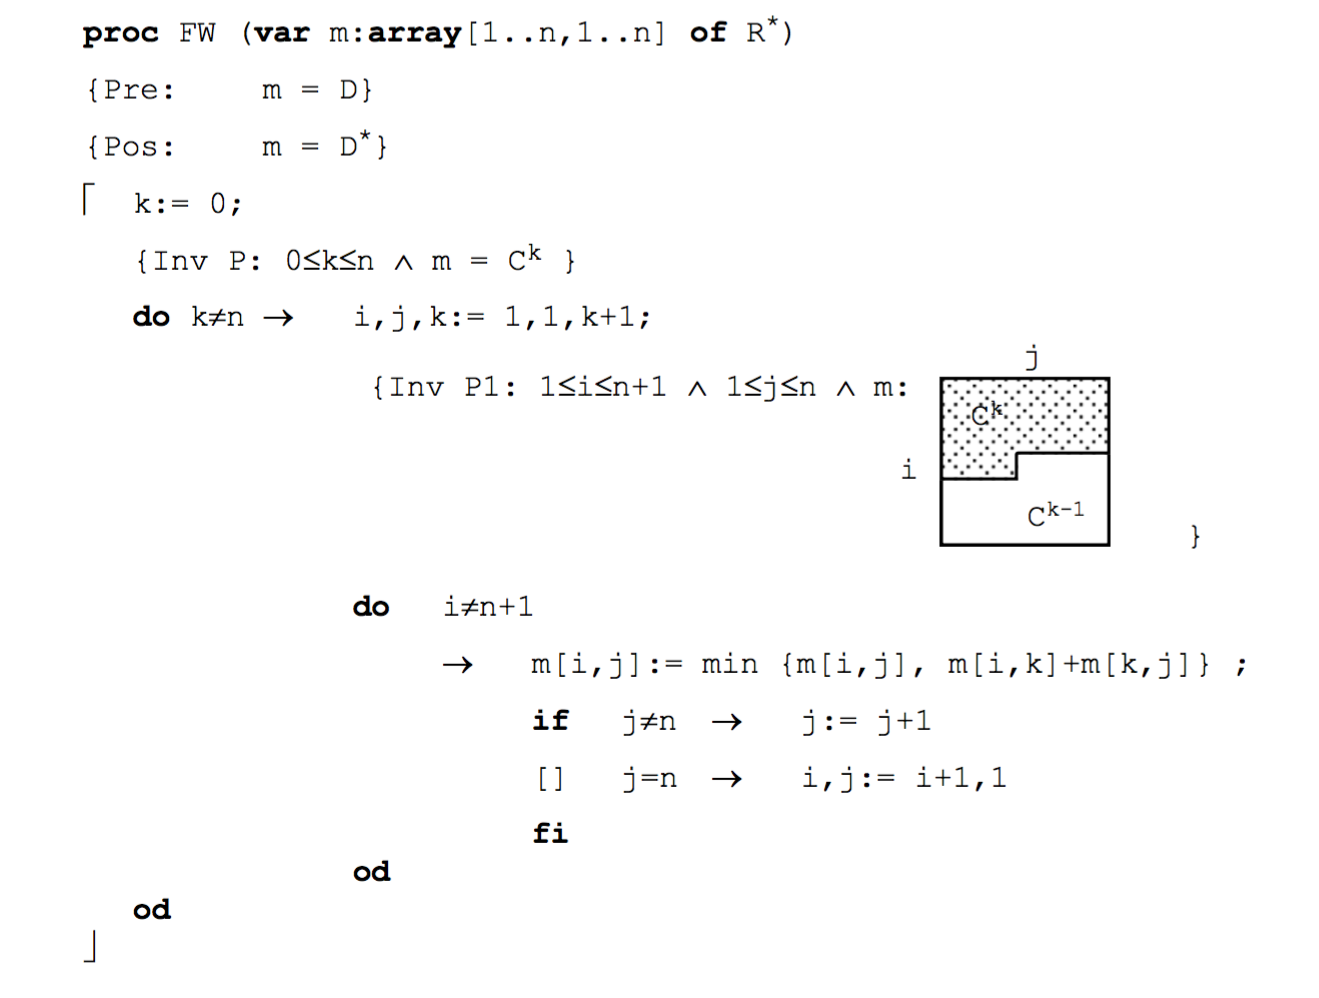
\includegraphics{FW.png}} 
 \caption{Floyd-Warshall ejemplo libro}
 \label{FW}
 \end{center}
\end{figure}
si se necesitara encontrar y reconstruir ese camino, se haria el mismo algoritmo, solo que actualizando una matriz tal que:

\begin{figure}[H]
\begin{center}
 \scalebox{0.5}{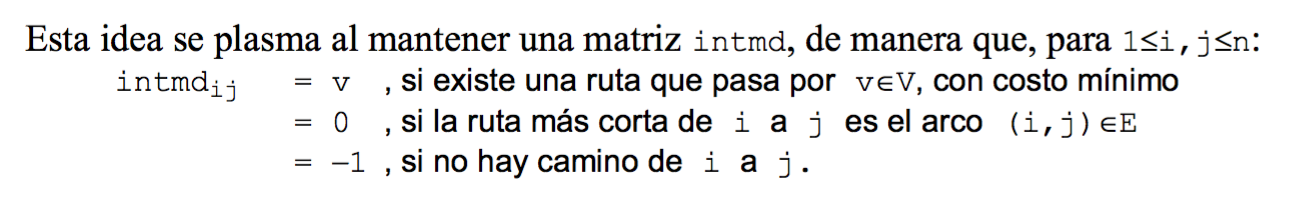
\includegraphics{intmd.png}} 
 \caption{Matriz para reconstruir el camino de costo minimo}
 \label{intmd}
 \end{center}
\end{figure}
 
 Para la complejidad temporal podemos encontrarla facilmente, como vemos en el algoritmo variamos i, j y k hasta n, donde n es el numero total de Nodos, y $T_{FW}=O(n^3)$, para la comlejidad Espacial tenemos guardamos una matriz de $nxn$ y es por esto que $S_{FW}=O(n^2)$

\subsubsection*{Dijkstra}
el algoritmo que me encuentra la ruta optima de un nodo f hasta el resto de nodos es: 

\begin{figure}[H]
\begin{center}
 \scalebox{0.5}{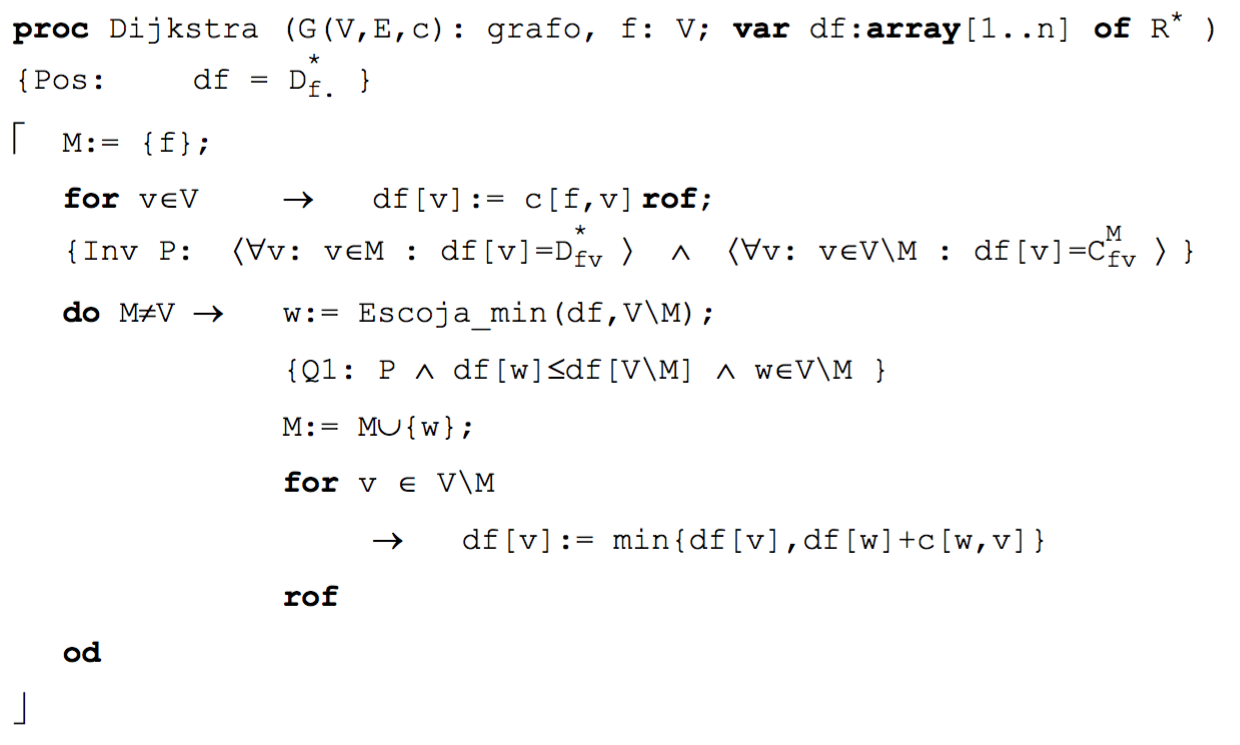
\includegraphics{dijkstra.png}} 
 \caption{Algoritmo de Dijkstra}
 \label{dijkstra}
 \end{center}
\end{figure}

donde la complejidad temporal depende de dos partes, la inicializacion y las iteraciones, la inicializacion es el primer for que llena el df, y las iteraciones son los ciclos que siguen.
\begin{equation}
T_D=T(Ini)+T(ciclos)=O(n)+O(n)[T(Escoja_min)+T(eliminar)]+O(e)
\end{equation}
Donde $T(Escoja_min)=O(n)$, ya que existen n diferentes nodos, teniendo todo en cuenta se obtiene que
\begin{equation}
T_D=O(n)[O(n)]+O(e)=O(n^2+e)
\end{equation}
pero esta seria la complejidad temporal para encontrar el camino minimo de un nodo dado f a el resto de los nodos del grafo, para obtener la totalidad de caminos minimos de todos los nodos hacia todos los nodos, debemos hacer este proceso para todos los nodos, en este casi la complejidad seria entonces:
\begin{equation}
T_{TD}=O(n(n^2+e))=O(n^3)
\end{equation}
donde se asumio que $e\ll n^3$, y para la espacial se guardara n vectores de la manera $di:i\in{1..f..n}$, y de esta manera $S_D=O(n^2)$


\subsection*{Punto 2}

\subsubsection*{2.a}
[para evitar errores se tiene que las vasijas seran $va_i$]Para modelar este problema de esta manera tenemos un grafo $G(V,E)$, con $V:= \{<v_1,..,v_n>|0\leq v_1 \leq c_1,..,0\leq v_n \leq c_n\}$ y debemos definir cuando se llega a un estado de solucion, y esto pasa cuando:
\begin{equation}
v_{final}\in V| v_k=P, k\in {1..n}
\end{equation}
y los arcos se definen como los cambios que se hacen en los estados de las vasijas, asi:
\begin{equation}
<v_1,..,v_n>\rightarrow_{accion} <v_1',..,v_n'>
\end{equation}
y accion sera el cambio que se hagan en las vasijas, y como las acciones que se pueden realizar son llenado y trasvasado tenemos que:

\begin{equation}
<v_1,..,v_n>\rightarrow_{Lk} <v_1,..,c_k,..,v_n>
\end{equation}
\begin{equation}
<v_1,..,v_n>\rightarrow_{Tki} \left\{ \begin{array}{lcc}
             <v_1,..,0,..,v_i+v_k,..,v_n> &   si  & v_i+v_k\leq c_i \\
             \\ <v_1,..,0,..,c_i,..,v_n> &  si & v_i+v_k\geq c_i 
              
             \end{array}
   \right.
\end{equation}
\subsubsection*{2.b}
Haremos uns busqueda en el grafo, y se buscara $v_{final} \in V$ una solucion que cumpla con la condicion anterior, apartir de un nodo $v_{inicial} \in V$.
\paragraph{Floyd-Marshall}



\subsection*{Punto 3}
Para este punto se deben notar un par de cosas interesantes, si $A=\{a_1,..,a_n\}$ es el conjunto de actividades, si escogemos un $a_i$ arbitrario, conocemos $B_i$, como $a_i \notin B_i$, ya que $B_i$ son las actividades que deben hacerce antes de $a_i$.
lo anterior nos lleva a decir que sea $a_k$ la ultima actividad a realizar, $|B_k|<n$, y una afirmacion mas fuerte aun pero igual de valida, $|B_k|=n-1$, $B_k+\{a_k\}=A$.
Para saber si el proyecto se puede hacer, se debe poder ordenar $A=\{a_k\}+\cup_{i=1}^{n} B_i$, con $|B_{i+1}|-|B_i|=1$. y es por esto que el problema se reduce a ordenar A y despues validar si estan las n actividades.
en el programa se usara la funcion $C(a_i)=B_i$, que me retorna el conjunto de actividades previas a $a_i$.
se ordenara una lista con la funcion $Orden(A)$ que me entrega $A'$ ordenado mediante seleccion, comparando el valor de $|C(a_i)|$, este ordenamiento tiene la complejidad normal para este algoritmo de ordenamiento $T=O(n^2)$
veamos como nos queda $A'$
\begin{equation}
Orden(A)=A'=[a'_1..a'_n], \text{ donde se cumple que: } |C(a'_1)|<..<|C(a'_n)|
\end{equation}
El algoritmo es:
\\\\
proc actividad (A=[$a_1..a_n$])  \\
A':=Orden(A);\\
po,i:=true,1;\\
do i $<$ n $\rightarrow$ $x,y:=|C(A'[i]|,|C(A'[i+1]|$;\\
\tab \tab IF $y-x\neq 1 \rightarrow po=\text{false }$FI\\
od\\
$\{$Pos: po=true $\bigvee$ po=false $\}$
Para la complejidad del algoritmo es la siguiente:
\begin{equation}
T_3=T(Orden)+T(ciclo)=O(n^2)+O(n)=O(n^2)
\end{equation}
\end{document}
